\chapter{الگوریتم‌های درخت}

\index{درخت}

یک \key{درخت} گرافی همبند و بدون دور است
که شامل $n$ رأس و $n-1$ یال می‌باشد.
حذف هر یال از یک درخت، آن را
به دو مؤلفه تقسیم می‌کند،
و اضافه کردن هر یال به درخت، یک دور ایجاد می‌نماید.
علاوه بر این، همواره یک مسیر یکتا بین هر
دو رأس از درخت وجود دارد.

برای مثال، درخت زیر از ۸ رأس و ۷ یال تشکیل شده است:
\begin{center}
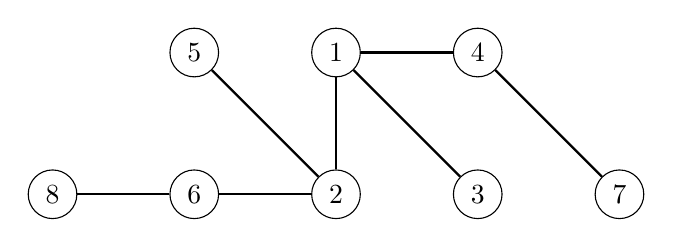
\begin{tikzpicture}[scale=0.9]
\node[draw, circle] (1) at (0,3) {$1$};
\node[draw, circle] (2) at (2,3) {$4$};
\node[draw, circle] (3) at (0,1) {$2$};
\node[draw, circle] (4) at (2,1) {$3$};
\node[draw, circle] (5) at (4,1) {$7$};
\node[draw, circle] (6) at (-2,3) {$5$};
\node[draw, circle] (7) at (-2,1) {$6$};
\node[draw, circle] (8) at (-4,1) {$8$};
\path[draw,thick,-] (1) -- (2);
\path[draw,thick,-] (1) -- (3);
\path[draw,thick,-] (1) -- (4);
\path[draw,thick,-] (2) -- (5);
\path[draw,thick,-] (3) -- (6);
\path[draw,thick,-] (3) -- (7);
\path[draw,thick,-] (7) -- (8);
\end{tikzpicture}
\end{center}

\index{برگ}

\key{برگ‌های} یک درخت، رأس‌هایی
با درجه‌ی ۱ هستند، یعنی فقط یک همسایه دارند.
برای مثال، برگ‌های درخت بالا
رأس‌های ۳، ۵، ۷ و ۸ هستند.

\index{ریشه}
\index{درخت ریشه‌دار}

در یک درخت \key{ریشه‌دار}، یکی از رأس‌ها
به عنوان \key{ریشه} درخت تعیین می‌شود،
و تمام رأس‌های دیگر
زیر ریشه قرار می‌گیرند.
برای مثال، در درخت زیر،
رأس ۱ ریشه است.

\begin{center}
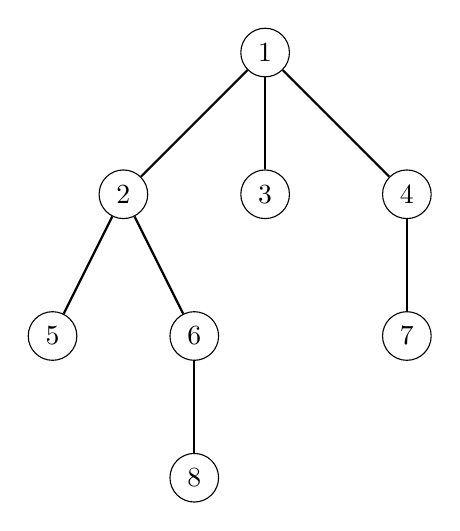
\begin{tikzpicture}[scale=0.9]
\node[draw, circle] (1) at (0,3) {$1$};
\node[draw, circle] (4) at (2,1) {$4$};
\node[draw, circle] (2) at (-2,1) {$2$};
\node[draw, circle] (3) at (0,1) {$3$};
\node[draw, circle] (7) at (2,-1) {$7$};
\node[draw, circle] (5) at (-3,-1) {$5$};
\node[draw, circle] (6) at (-1,-1) {$6$};
\node[draw, circle] (8) at (-1,-3) {$8$};
\path[draw,thick,-] (1) -- (2);
\path[draw,thick,-] (1) -- (3);
\path[draw,thick,-] (1) -- (4);
\path[draw,thick,-] (2) -- (5);
\path[draw,thick,-] (2) -- (6);
\path[draw,thick,-] (4) -- (7);
\path[draw,thick,-] (6) -- (8);
\end{tikzpicture}
\end{center}
\index{فرزند}
\index{والد}

در یک درخت ریشه‌دار، \key{فرزندان} یک رأس
همسایه‌های پایینی آن هستند، و \key{والد} یک رأس
همسایه‌ی بالایی آن است.
هر رأس دقیقاً یک والد دارد،
به جز ریشه که والدی ندارد.
برای مثال، در درخت بالا،
فرزندان رأس ۲ رأس‌های ۵ و ۶ هستند،
و والد آن رأس ۱ است.

\index{زیردرخت}

ساختار درخت ریشه‌دار \emph{بازگشتی} است:
هر گره درخت، ریشه یک \key{زیردرخت} است
که شامل خود گره و تمام گره‌های
موجود در زیردرخت‌های فرزندان آن است.
به عنوان مثال، در درخت بالا، زیردرخت گره ۲
شامل گره‌های ۲، ۵، ۶ و ۸ است:
\begin{center}
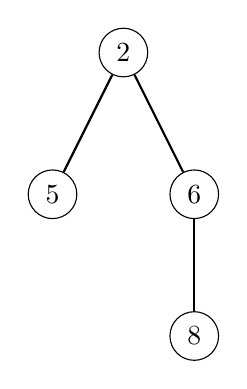
\begin{tikzpicture}[scale=0.9]
\node[draw, circle] (2) at (-2,1) {$2$};
\node[draw, circle] (5) at (-3,-1) {$5$};
\node[draw, circle] (6) at (-1,-1) {$6$};
\node[draw, circle] (8) at (-1,-3) {$8$};
\path[draw,thick,-] (2) -- (5);
\path[draw,thick,-] (2) -- (6);
\path[draw,thick,-] (6) -- (8);
\end{tikzpicture}
\end{center}

\section{پیمایش درخت}

الگوریتم‌های عمومی پیمایش گراف
می‌توانند برای پیمایش گره‌های یک درخت استفاده شوند.
با این حال، پیاده‌سازی پیمایش درخت ساده‌تر از
گراف عمومی است، زیرا
هیچ دوری در درخت وجود ندارد و رسیدن
به یک گره از چندین جهت ممکن نیست.

روش معمول پیمایش درخت، شروع
جستجوی اول-عمق از یک گره دلخواه است.
تابع بازگشتی زیر می‌تواند استفاده شود:

\begin{lstlisting}
void dfs(int s, int e) {
    // پردازش گره s
    for (auto u : adj[s]) {
        if (u != e) dfs(u, s);
    }
}
\end{lstlisting}

تابع دو پارامتر می‌گیرد: گره فعلی $s$
و گره قبلی $e$.
هدف پارامتر $e$ اطمینان از این است
که جستجو فقط به گره‌هایی حرکت کند
که هنوز بازدید نشده‌اند.

فراخوانی زیر جستجو را
از گره $x$ آغاز می‌کند:

\begin{lstlisting}
dfs(x, 0);
\end{lstlisting}

در فراخوانی اول $e=0$ است، زیرا هیچ
گره قبلی وجود ندارد و حرکت
به هر جهتی در درخت مجاز است.

\subsubsection{برنامه‌نویسی پویا}

برنامه‌نویسی پویا می‌تواند برای محاسبه
اطلاعات حین پیمایش درخت استفاده شود.
با استفاده از برنامه‌نویسی پویا می‌توان، برای مثال،
در زمان $O(n)$ برای هر گره درخت ریشه‌دار، تعداد
گره‌های زیردرخت آن
یا طول طولانی‌ترین مسیر از آن گره
تا یک برگ را محاسبه کرد.

به عنوان مثال، برای هر گره $s$
مقدار $\texttt{count}[s]$ را محاسبه می‌کنیم: تعداد گره‌های زیردرخت آن.
زیردرخت شامل خود گره و
تمام گره‌های زیردرخت‌های فرزندان آن است،
بنابراین می‌توان تعداد گره‌ها را
به صورت بازگشتی با کد زیر محاسبه کرد:

\begin{lstlisting}
void dfs(int s, int e) {
    count[s] = 1;
    for (auto u : adj[s]) {
        if (u == e) continue;
        dfs(u, s);
        count[s] += count[u];
    }
}
\end{lstlisting}

\section{قطر}

\index{قطر}

\key{قطر} یک درخت
بیشینه طول یک مسیر بین دو رأس است.
برای مثال، درخت زیر را در نظر بگیرید:
\begin{center}
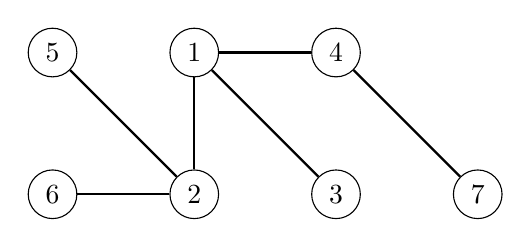
\begin{tikzpicture}[scale=0.9]
\node[draw, circle] (1) at (0,3) {$1$};
\node[draw, circle] (2) at (2,3) {$4$};
\node[draw, circle] (3) at (0,1) {$2$};
\node[draw, circle] (4) at (2,1) {$3$};
\node[draw, circle] (5) at (4,1) {$7$};
\node[draw, circle] (6) at (-2,3) {$5$};
\node[draw, circle] (7) at (-2,1) {$6$};
\path[draw,thick,-] (1) -- (2);
\path[draw,thick,-] (1) -- (3);
\path[draw,thick,-] (1) -- (4);
\path[draw,thick,-] (2) -- (5);
\path[draw,thick,-] (3) -- (6);
\path[draw,thick,-] (3) -- (7);
\end{tikzpicture}
\end{center}
قطر این درخت برابر ۴ است
که متناظر با مسیر زیر است:
\begin{center}
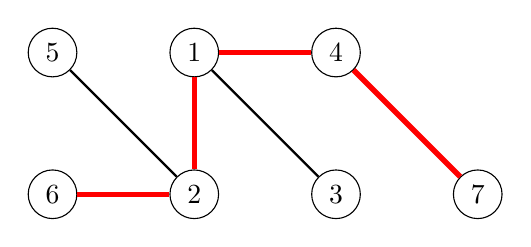
\begin{tikzpicture}[scale=0.9]
\node[draw, circle] (1) at (0,3) {$1$};
\node[draw, circle] (2) at (2,3) {$4$};
\node[draw, circle] (3) at (0,1) {$2$};
\node[draw, circle] (4) at (2,1) {$3$};
\node[draw, circle] (5) at (4,1) {$7$};
\node[draw, circle] (6) at (-2,3) {$5$};
\node[draw, circle] (7) at (-2,1) {$6$};
\path[draw,thick,-] (1) -- (2);
\path[draw,thick,-] (1) -- (3);
\path[draw,thick,-] (1) -- (4);
\path[draw,thick,-] (2) -- (5);
\path[draw,thick,-] (3) -- (6);
\path[draw,thick,-] (3) -- (7);

\path[draw,thick,-,color=red,line width=2pt] (7) -- (3);
\path[draw,thick,-,color=red,line width=2pt] (3) -- (1);
\path[draw,thick,-,color=red,line width=2pt] (1) -- (2);
\path[draw,thick,-,color=red,line width=2pt] (2) -- (5);
\end{tikzpicture}
\end{center}
توجه کنید ممکن است چندین مسیر با بیشینه طول وجود داشته باشد.
در مسیر بالا، می‌توان رأس ۶ را با رأس ۵ جایگزین کرد
تا مسیر دیگری با طول ۴ به دست آید.

در ادامه دو الگوریتم با زمان اجرای $O(n)$
برای محاسبه قطر درخت بررسی می‌شود.
الگوریتم نخست بر پایه برنامه‌نویسی پویا است
و الگوریتم دوم از دو پیمایش اول-عمق استفاده می‌کند.

\subsubsection{الگوریتم ۱}

یک روش کلی برای حل مسائل درخت
این است که ابتدا درخت را دلخواه ریشه‌دار کنیم.
پس از آن، می‌توان مسئله را
به‌طور جداگانه برای هر زیردرخت حل کرد.
الگوریتم نخست برای محاسبه قطر
بر پایه همین ایده است.

مشاهده مهم این است که هر مسیر
در یک درخت ریشه‌دار، یک \emph{بالاترین نقطه} دارد:
بالاترین رأسی که متعلق به مسیر است.
بنابراین، می‌توان برای هر رأس، طول
طولانی‌ترین مسیری را که بالاترین نقطه‌اش آن رأس است محاسبه کرد.
یکی از این مسیرها متناظر با قطر درخت خواهد بود.

برای مثال، در درخت زیر،
گره ۱ بالاترین نقطه در مسیری است
که متناظر با قطر است:
\begin{center}
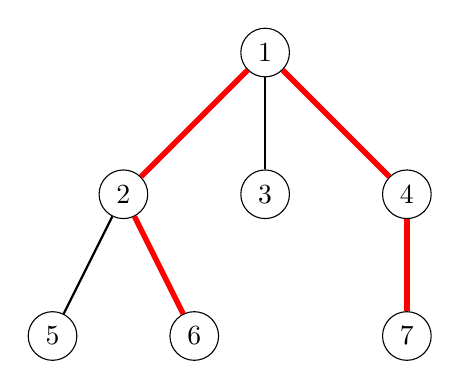
\begin{tikzpicture}[scale=0.9]
\node[draw, circle] (1) at (0,3) {$1$};
\node[draw, circle] (2) at (2,1) {$4$};
\node[draw, circle] (3) at (-2,1) {$2$};
\node[draw, circle] (4) at (0,1) {$3$};
\node[draw, circle] (5) at (2,-1) {$7$};
\node[draw, circle] (6) at (-3,-1) {$5$};
\node[draw, circle] (7) at (-1,-1) {$6$};
\path[draw,thick,-] (1) -- (2);
\path[draw,thick,-] (1) -- (3);
\path[draw,thick,-] (1) -- (4);
\path[draw,thick,-] (2) -- (5);
\path[draw,thick,-] (3) -- (6);
\path[draw,thick,-] (3) -- (7);

\path[draw,thick,-,color=red,line width=2pt] (7) -- (3);
\path[draw,thick,-,color=red,line width=2pt] (3) -- (1);
\path[draw,thick,-,color=red,line width=2pt] (1) -- (2);
\path[draw,thick,-,color=red,line width=2pt] (2) -- (5);
\end{tikzpicture}
\end{center}

برای هر گره $x$ دو مقدار محاسبه می‌کنیم:
\begin{itemize}
\item $\texttt{toLeaf}(x)$: بیشینه طول مسیر از $x$ به هر برگ
\item $\texttt{maxLength}(x)$: بیشینه طول مسیری
که بالاترین نقطه آن $x$ است
\end{itemize}
برای مثال، در درخت بالا،
$\texttt{toLeaf}(1)=2$، زیرا مسیر
$1 \rightarrow 2 \rightarrow 6$ وجود دارد،
و $\texttt{maxLength}(1)=4$،
زیرا مسیر
$6 \rightarrow 2 \rightarrow 1 \rightarrow 4 \rightarrow 7$ وجود دارد.
در این حالت، $\texttt{maxLength}(1)$ برابر با قطر است.

می‌توان از برنامه‌نویسی پویا برای محاسبه مقادیر بالا
برای همه گره‌ها در زمان $O(n)$ استفاده کرد.
ابتدا برای محاسبه $\texttt{toLeaf}(x)$،
فرزندان $x$ را بررسی می‌کنیم،
فرزند $c$ با بیشینه $\texttt{toLeaf}(c)$ را انتخاب کرده
و یک واحد به این مقدار اضافه می‌کنیم.
سپس برای محاسبه $\texttt{maxLength}(x)$،
دو فرزند متمایز $a$ و $b$ را طوری انتخاب می‌کنیم
که مجموع $\texttt{toLeaf}(a)+\texttt{toLeaf}(b)$
بیشینه باشد و دو واحد به این مجموع اضافه می‌کنیم.

\subsubsection{الگوریتم ۲}

روش کارآمد دیگر برای محاسبه قطر
درخت مبتنی بر دو بار جستجوی اول عمق است.
ابتدا یک گره دلخواه $a$ در درخت انتخاب می‌کنیم
و دورترین گره $b$ از $a$ را می‌یابیم.
سپس دورترین گره $c$ از $b$ را پیدا می‌کنیم.
قطر درخت فاصله بین $b$ و $c$ است.

در گراف زیر، $a$، $b$ و $c$ می‌توانند به این صورت باشند:
\begin{center}
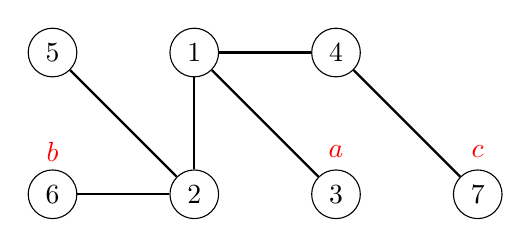
\begin{tikzpicture}[scale=0.9]
\node[draw, circle] (1) at (0,3) {$1$};
\node[draw, circle] (2) at (2,3) {$4$};
\node[draw, circle] (3) at (0,1) {$2$};
\node[draw, circle] (4) at (2,1) {$3$};
\node[draw, circle] (5) at (4,1) {$7$};
\node[draw, circle] (6) at (-2,3) {$5$};
\node[draw, circle] (7) at (-2,1) {$6$};
\path[draw,thick,-] (1) -- (2);
\path[draw,thick,-] (1) -- (3);
\path[draw,thick,-] (1) -- (4);
\path[draw,thick,-] (2) -- (5);
\path[draw,thick,-] (3) -- (6);
\path[draw,thick,-] (3) -- (7);
\node[color=red] at (2,1.6) {$a$};
\node[color=red] at (-2,1.6) {$b$};
\node[color=red] at (4,1.6) {$c$};
\end{tikzpicture}
\end{center}

\path[draw,thick,-,color=red,line width=2pt] (7) -- (3);
\path[draw,thick,-,color=red,line width=2pt] (3) -- (1);
\path[draw,thick,-,color=red,line width=2pt] (1) -- (2);
\path[draw,thick,-,color=red,line width=2pt] (2) -- (5);
\end{tikzpicture}
\end{center}

روش هوشمندانه است، اما چرا کار می‌کند؟

رسم متفاوت درخت فهم را ساده می‌کند؛ طوری که مسیر متناظر با قطر، افقی باشد و باقی رأس‌ها از آن آویزان شوند:
\begin{center}
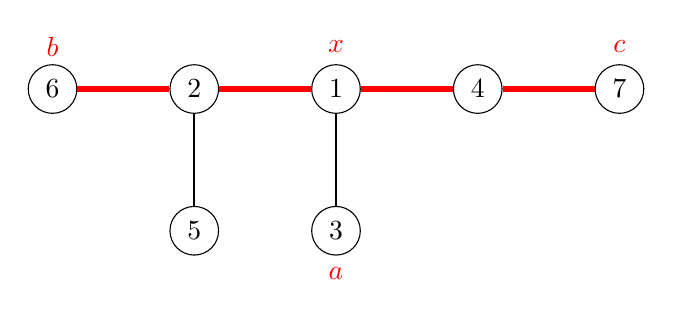
\begin{tikzpicture}[scale=0.9]
\node[draw, circle] (1) at (2,1) {$1$};
\node[draw, circle] (2) at (4,1) {$4$};
\node[draw, circle] (3) at (0,1) {$2$};
\node[draw, circle] (4) at (2,-1) {$3$};
\node[draw, circle] (5) at (6,1) {$7$};
\node[draw, circle] (6) at (0,-1) {$5$};
\node[draw, circle] (7) at (-2,1) {$6$};
\path[draw,thick,-] (1) -- (2);
\path[draw,thick,-] (1) -- (3);
\path[draw,thick,-] (1) -- (4);
\path[draw,thick,-] (2) -- (5);
\path[draw,thick,-] (3) -- (6);
\path[draw,thick,-] (3) -- (7);
\node[color=red] at (2,-1.6) {$a$};
\node[color=red] at (-2,1.6) {$b$};
\node[color=red] at (6,1.6) {$c$};
\node[color=red] at (2,1.6) {$x$};

\path[draw,thick,-,color=red,line width=2pt] (7) -- (3);
\path[draw,thick,-,color=red,line width=2pt] (3) -- (1);
\path[draw,thick,-,color=red,line width=2pt] (1) -- (2);
\path[draw,thick,-,color=red,line width=2pt] (2) -- (5);
\end{tikzpicture}
\end{center}

رأس $x$ محل اتصال مسیر مبدأ $a$ به مسیر قطر است.
دورترین رأس از $a$، رأس $b$، رأس $c$ یا رأسی دیگر با دست‌کم همین فاصله از $x$ است.
بنابراین، این رأس همیشه انتخابی معتبر برای یک سر مسیر قطر است.

\section{همه طولانی‌ترین مسیرها}

مسئله بعدی: محاسبه بیشینه طول مسیر شروع‌شده از هر رأس درخت.
این تعمیم مسئله قطر درخت است، چون بیشینه این مقادیر برابر قطر درخت است.
حل در زمان $O(n)$ ممکن است.

مثال، درخت زیر:
\begin{center}
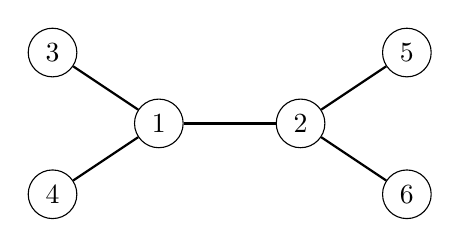
\begin{tikzpicture}[scale=0.9]
\node[draw, circle] (1) at (0,0) {$1$};
\node[draw, circle] (2) at (-1.5,-1) {$4$};
\node[draw, circle] (3) at (2,0) {$2$};
\node[draw, circle] (4) at (-1.5,1) {$3$};
\node[draw, circle] (6) at (3.5,-1) {$6$};
\node[draw, circle] (7) at (3.5,1) {$5$};
\path[draw,thick,-] (1) -- (2);
\path[draw,thick,-] (1) -- (3);
\path[draw,thick,-] (1) -- (4);
\path[draw,thick,-] (3) -- (6);
\path[draw,thick,-] (3) -- (7);
\end{tikzpicture}
\end{center}

فرض کنید $\texttt{maxLength}(x)$ بیشینه طول مسیر با شروع از رأس $x$ باشد.
در درخت بالا، $\texttt{maxLength}(4)=3$ است، چون مسیر $4 \rightarrow 1 \rightarrow 2 \rightarrow 6$ وجود دارد.
جدول کامل مقادیر:
\begin{center}
\begin{tabular}{l|lllllll}
رأس $x$ & 1 & 2 & 3 & 4 & 5 & 6 \\
$\texttt{maxLength}(x)$ & 2 & 2 & 3 & 3 & 3 & 3 \\
\end{tabular}
\end{center}

همچنین در این مسئله، یک نقطه شروع خوب برای حل، ریشه‌دار کردن دلخواه درخت است:
\begin{center}
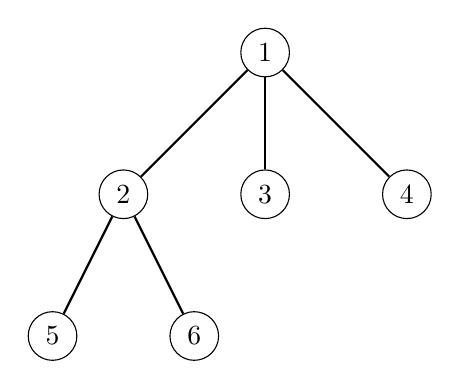
\begin{tikzpicture}[scale=0.9]
\node[draw, circle] (1) at (0,3) {$1$};
\node[draw, circle] (2) at (2,1) {$4$};
\node[draw, circle] (3) at (-2,1) {$2$};
\node[draw, circle] (4) at (0,1) {$3$};
\node[draw, circle] (6) at (-3,-1) {$5$};
\node[draw, circle] (7) at (-1,-1) {$6$};
\path[draw,thick,-] (1) -- (2);
\path[draw,thick,-] (1) -- (3);
\path[draw,thick,-] (1) -- (4);
\path[draw,thick,-] (3) -- (6);
\path[draw,thick,-] (3) -- (7);
\end{tikzpicture}
\end{center}

بخش اول مسئله، محاسبه بیشترین طول مسیری است که به ازای هر گره $x$، از یکی از فرزندان $x$ عبور می‌کند.
برای نمونه، طولانی‌ترین مسیر از گره 1 از فرزند آن، یعنی 2، می‌گذرد:
\begin{center}
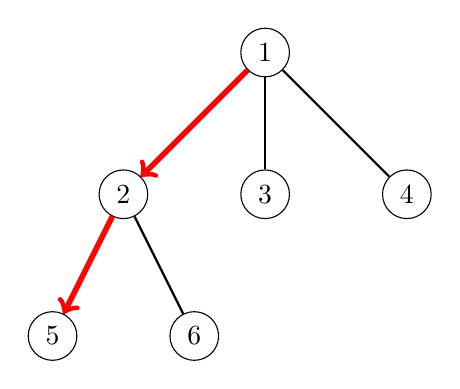
\begin{tikzpicture}[scale=0.9]
\node[draw, circle] (1) at (0,3) {$1$};
\node[draw, circle] (2) at (2,1) {$4$};
\node[draw, circle] (3) at (-2,1) {$2$};
\node[draw, circle] (4) at (0,1) {$3$};
\node[draw, circle] (6) at (-3,-1) {$5$};
\node[draw, circle] (7) at (-1,-1) {$6$};
\path[draw,thick,-] (1) -- (2);
\path[draw,thick,-] (1) -- (3);
\path[draw,thick,-] (1) -- (4);
\path[draw,thick,-] (3) -- (6);
\path[draw,thick,-] (3) -- (7);

\path[draw,thick,->,color=red,line width=2pt] (1) -- (3);
\path[draw,thick,->,color=red,line width=2pt] (3) -- (6);
\end{tikzpicture}
\end{center}
حل این بخش در زمان $O(n)$ ساده است، زیرا می‌توان مانند گذشته از برنامه‌نویسی پویا استفاده کرد.

سپس، بخش دوم مسئله محاسبه بیشترین طول مسیر از طریق والد $p$ به ازای هر گره $x$ است.
برای نمونه، طولانی‌ترین مسیر از گره 3 از والد آن، یعنی 1، می‌گذرد:
\begin{center}
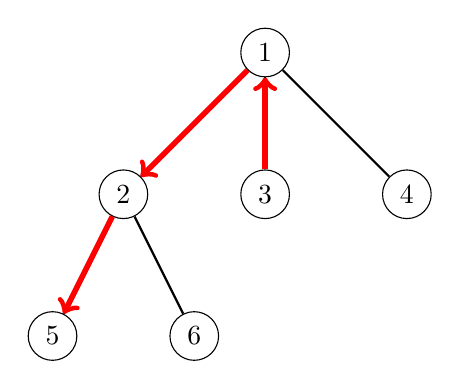
\begin{tikzpicture}[scale=0.9]
\node[draw, circle] (1) at (0,3) {$1$};
\node[draw, circle] (2) at (2,1) {$4$};
\node[draw, circle] (3) at (-2,1) {$2$};
\node[draw, circle] (4) at (0,1) {$3$};
\node[draw, circle] (6) at (-3,-1) {$5$};
\node[draw, circle] (7) at (-1,-1) {$6$};
\path[draw,thick,-] (1) -- (2);
\path[draw,thick,-] (1) -- (3);
\path[draw,thick,-] (1) -- (4);
\path[draw,thick,-] (3) -- (6);
\path[draw,thick,-] (3) -- (7);

\path[draw,thick,->,color=red,line width=2pt] (4) -- (1);
\path[draw,thick,->,color=red,line width=2pt] (1) -- (3);
\path[draw,thick,->,color=red,line width=2pt] (3) -- (6);
\end{tikzpicture}
\end{center}

در نگاه اول، به نظر می‌رسد باید
طولانی‌ترین مسیر از $p$ را انتخاب کنیم.
اما این روش همیشه کار \emph{نمی‌کند}،
زیرا ممکن است طولانی‌ترین مسیر از $p$
از $x$ عبور کند.
نمونه‌ای از این وضعیت:
\begin{center}
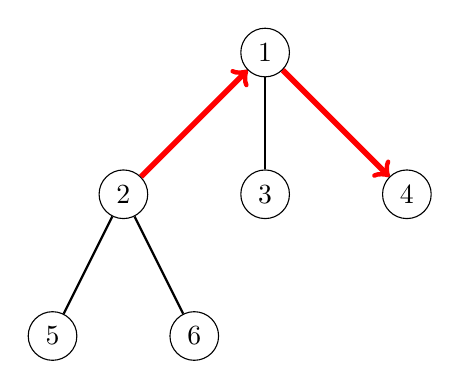
\begin{tikzpicture}[scale=0.9]
\node[draw, circle] (1) at (0,3) {$1$};
\node[draw, circle] (2) at (2,1) {$4$};
\node[draw, circle] (3) at (-2,1) {$2$};
\node[draw, circle] (4) at (0,1) {$3$};
\node[draw, circle] (6) at (-3,-1) {$5$};
\node[draw, circle] (7) at (-1,-1) {$6$};
\path[draw,thick,-] (1) -- (2);
\path[draw,thick,-] (1) -- (3);
\path[draw,thick,-] (1) -- (4);
\path[draw,thick,-] (3) -- (6);
\path[draw,thick,-] (3) -- (7);

\path[draw,thick,->,color=red,line width=2pt] (3) -- (1);
\path[draw,thick,->,color=red,line width=2pt] (1) -- (2);
\end{tikzpicture}
\end{center}

با این حال، می‌توان بخش دوم را در
زمان $O(n)$ با ذخیره \emph{دو} بیشینه طول
برای هر رأس $x$ حل کرد:
\begin{itemize}
\item $\texttt{maxLength}_1(x)$:
بیشینه طول یک مسیر از $x$
\item $\texttt{maxLength}_2(x)$:
بیشینه طول یک مسیر از $x$
در جهتی متفاوت از مسیر اول
\end{itemize}
به عنوان مثال، در گراف بالا،
$\texttt{maxLength}_1(1)=2$
با استفاده از مسیر $1 \rightarrow 2 \rightarrow 5$،
و $\texttt{maxLength}_2(1)=1$
با استفاده از مسیر $1 \rightarrow 3$.

در نهایت، اگر مسیر متناظر با
$\texttt{maxLength}_1(p)$ از $x$ بگذرد،
نتیجه می‌گیریم بیشینه طول برابر است با
$\texttt{maxLength}_2(p)+1$،
و در غیر این صورت بیشینه طول برابر است با
$\texttt{maxLength}_1(p)+1$.


\section{درخت‌های دودویی}

\index{درخت دودویی}

\begin{samepage}
یک \key{درخت دودویی} درختی ریشه‌دار است
که هر رأس آن یک زیردرخت چپ و راست دارد.
امکان تهی بودن زیردرخت یک رأس وجود دارد.
بنابراین، هر رأس در درخت دودویی
صفر، یک یا دو فرزند دارد.

برای نمونه، درخت زیر یک درخت دودویی است:
\begin{center}
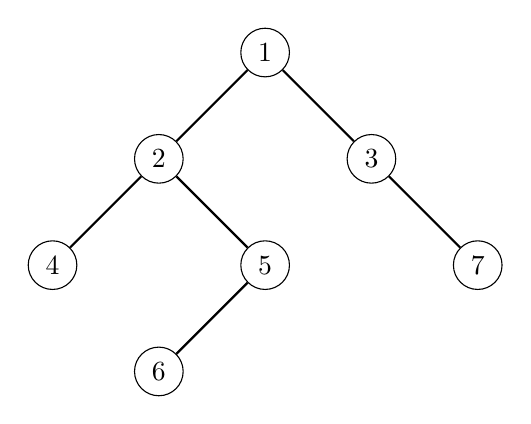
\begin{tikzpicture}[scale=0.9]
\node[draw, circle] (1) at (0,0) {$1$};
\node[draw, circle] (2) at (-1.5,-1.5) {$2$};
\node[draw, circle] (3) at (1.5,-1.5) {$3$};
\node[draw, circle] (4) at (-3,-3) {$4$};
\node[draw, circle] (5) at (0,-3) {$5$};
\node[draw, circle] (6) at (-1.5,-4.5) {$6$};
\node[draw, circle] (7) at (3,-3) {$7$};

\path[draw,thick,-] (1) -- (2);
\path[draw,thick,-] (1) -- (3);
\path[draw,thick,-] (2) -- (4);
\path[draw,thick,-] (2) -- (5);
\path[draw,thick,-] (5) -- (6);
\path[draw,thick,-] (3) -- (7);
\end{tikzpicture}
\end{center}
\end{samepage}

\index{پیش‌ترتیب}
\index{میان‌ترتیب}
\index{پس‌ترتیب}

رأس‌های درخت دودویی دارای سه ترتیب طبیعی هستند
که متناظر با روش‌های مختلف پیمایش بازگشتی
درخت است:

\begin{itemize}
\item \key{پیش‌ترتیب}: ابتدا پردازش ریشه،
سپس پیمایش زیردرخت چپ، سپس پیمایش زیردرخت راست
\item \key{میان‌ترتیب}: ابتدا پیمایش زیردرخت چپ،
سپس پردازش ریشه، سپس پیمایش زیردرخت راست
\item \key{پس‌ترتیب}: ابتدا پیمایش زیردرخت چپ،
سپس پیمایش زیردرخت راست، سپس پردازش ریشه
\end{itemize}

برای درخت بالا، گره‌ها در
پیمایش پیش‌ترتیب
$[1,2,4,5,6,3,7]$،
در میان‌ترتیب $[4,2,6,5,1,3,7]$
و در پس‌ترتیب $[4,6,5,2,7,3,1]$ هستند.

اگر پیش‌ترتیب و میان‌ترتیب درختی معلوم باشد، می‌توان ساختار دقیق درخت را بازسازی کرد.
برای نمونه، درخت بالا تنها درخت ممکن با
پیش‌ترتیب $[1,2,4,5,6,3,7]$ و
میان‌ترتیب $[4,2,6,5,1,3,7]$ است.
به شیوه مشابه، پس‌ترتیب و میان‌ترتیب نیز ساختار درخت را تعیین می‌کنند.

با این حال، اگر تنها پیش‌ترتیب و پس‌ترتیب درخت معلوم باشد، وضعیت متفاوت است.
در این حالت، ممکن است بیش از یک درخت با این ترتیب‌ها همخوانی داشته باشد.
برای نمونه، در هر دوی درخت‌های
\begin{center}
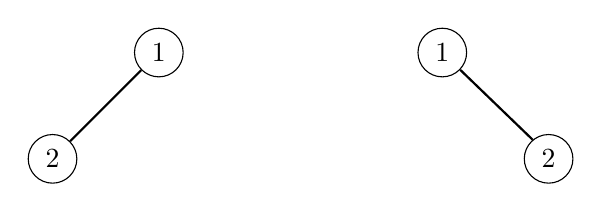
\begin{tikzpicture}[scale=0.9]
\node[draw, circle] (1) at (0,0) {$1$};
\node[draw, circle] (2) at (-1.5,-1.5) {$2$};
\path[draw,thick,-] (1) -- (2);

\node[draw, circle] (1b) at (0+4,0) {$1$};
\node[draw, circle] (2b) at (1.5+4,-1.5) {$2$};
\path[draw,thick,-] (1b) -- (2b);
\end{tikzpicture}
\end{center}
پیش‌ترتیب $[1,2]$ و پس‌ترتیب $[2,1]$ است،
اما ساختار درخت‌ها با یکدیگر تفاوت دارد.